\documentclass{article}
\usepackage[utf8]{inputenc}
\usepackage{graphicx}
\usepackage{mathtools}
\usepackage{amsmath}

\title{Backpropagation e o método do gradiente}

\author{Frederico José Ribeiro Pelogia}


\date{October 2019}

\begin{document}

\maketitle
\section{Método do gradiente}

É um dos métodos mais clássicos no estudo de otimização. O método é iterativo e consiste em avançar, a partir de um ponto inicial, na direção oposta à do gradiente da função neste ponto, isto é, na direção de maior decrescimento. O tamanho do passo (t) deve ser definido de modo que o ponto $x^{k+1}$ esteja mais próximo da solução (do mínimo da função) do que $x^k$.

Basicamente:

$$
    \large x^{k+1} = x^k - t^k \nabla f(x^k)
$$
\subsection{Aplicando o método do gradiente no treinamento de redes neurais} \label{mgradnn}

Seja uma rede neural com a arquitetura apresentada na Figura \ref{fig:network}.

\begin{figure}[h]
\centering 
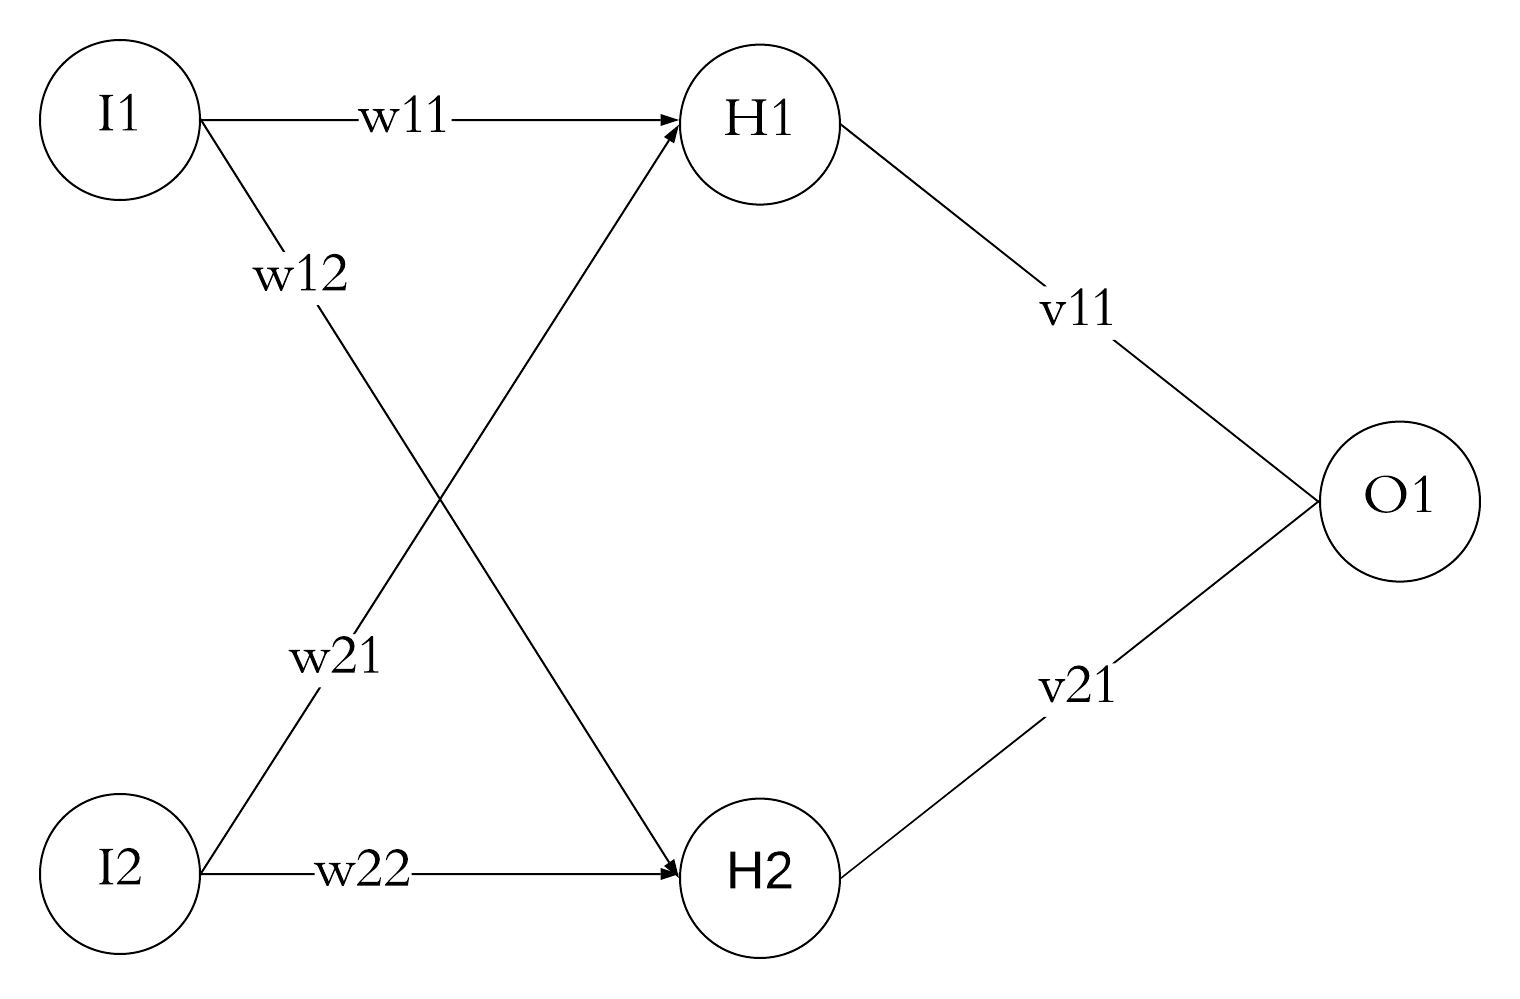
\includegraphics[scale = 0.3]{network.png}
\caption{Arquitetura da rede} \label{fig:network}
\end{figure}

Definiremos $I$ como a camada de entrada, $H$ como a camada oculta, $O$ como a camada de saída, W como a matriz de pesos entre $I$ e $H$, e V como a matriz de pesos entre $H$ e $O$. Seja $f_{h}$ a função de ativação da camada $H$ e $f_{o}$ a função de ativação da camada $O$.

A alimentação da rede, para que ela gere uma resposta a partir de um dado de treinamento, funciona da seguiunte maneira:

$$
    I = \begin{pmatrix}I_1\\I_2\end{pmatrix}, H = \begin{pmatrix}H_1\\H_2\end{pmatrix}, O = \begin{pmatrix}O_1\end{pmatrix}, 
    W = \begin{pmatrix}w_{11}&w_{21}\\w_{12}&w_{22}\end{pmatrix}, V = \begin{pmatrix}v_{11}&v_{21}\end{pmatrix}
$$

$$
    H_{in} = W \cdot I = \begin{pmatrix}w_{11}&w_{21}\\w_{12}&w_{22}\end{pmatrix} \cdot \begin{pmatrix}I_1\\I_{2}\end{pmatrix} = \begin{pmatrix}w_{11}I_1 + w_{21}I_2 \\ w_{12}I_1 + w_{22}I_2 \end{pmatrix}
$$   

$$
    \implies H = f_h(H_{in})=\begin{pmatrix}f_h(w_{11}I_1 + w_{21}I_2) \\ f_h(w_{12}I_1 + w_{22}I_2) \end{pmatrix}
$$    

$$  
    O_{in} = V \cdot H = \begin{pmatrix}v_{11}&v_{21}\end{pmatrix} \cdot \begin{pmatrix}H_1\\H_2\end{pmatrix} =  
    = v_{11}f_h(w_{11}I_1 + w_{21}I_2) + v_{21}f_h(w_{12}I_1 + w_{22}I_2)
    \implies O = f_o(O_{in}) = f_o(v_{11}f_h(w_{11}I_1 + w_{21}I_2) + v_{21}f_h(w_{12}I_1 + w_{22}I_2))
$$


Agora, tendo o \textit{output} da rede para o exemplo de treinamento e a resposta correta (\textit{label}) $y$, podemos montar uma função $EQ$ que represente o erro quadrático da predição.


$$
    EQ\begin{pmatrix}w_{11}\\\vdots\\v_{21}\end{pmatrix} = \frac{1}{2}(O\begin{pmatrix}I_{1}\\ \vdots \\v_{21} \end{pmatrix} - (y))^2
$$
\\

Agora, analisemos as derivadas parciais dessa função em relação a cada um dos pesos a serem otimizados mais tarde:

Seja
$$ E\begin{pmatrix}w_{11}\\\vdots\\v_{21}\end{pmatrix} = (O\begin{pmatrix}I_{1}\\ \vdots \\v_{21} \end{pmatrix} - (y))
$$

$$
    \frac{\partial EQ}{\partial w_{11}}\begin{pmatrix}w_{11}\\\vdots\\v_{21}\end{pmatrix} = E\begin{pmatrix}I_{1}\\ \vdots \\v_{11} \end{pmatrix}\cdot f_o'(O_{in})\cdot v_{11} \cdot f_h'(H_{1})\cdot I_{1}
$$
$$
    \frac{\partial EQ}{\partial w_{12}}\begin{pmatrix}w_{11}\\\vdots\\v_{21}\end{pmatrix} = E\begin{pmatrix}I_{1}\\ \vdots \\v_{21} \end{pmatrix}\cdot f_o'(O_{in})\cdot v_{21} \cdot f_h'(H_{2})\cdot I_{1}
$$
$$
    \frac{\partial EQ}{\partial w_{21}}\begin{pmatrix}w_{11}\\\vdots\\v_{21}\end{pmatrix} = E\begin{pmatrix}I_{1}\\ \vdots \\v_{21} \end{pmatrix}\cdot f_o'(O_{in})\cdot v_{11} \cdot f_h'(H_{1})\cdot I_{2}
$$
$$
    \frac{\partial EQ}{\partial w_{22}}\begin{pmatrix}w_{11}\\\vdots\\v_{21}\end{pmatrix} = E\begin{pmatrix}I_{1}\\ \vdots \\v_{21} \end{pmatrix}\cdot f_o'(O_{in})\cdot v_{21} \cdot f_h'(H_{2})\cdot I_{2}
$$

$$
    \frac{\partial EQ}{\partial v_{11}}\begin{pmatrix}w_{11}\\\vdots\\v_{21}\end{pmatrix} = E\begin{pmatrix}I_{1}\\ \vdots \\v_{21} \end{pmatrix}\cdot f_o'(O_{in})\cdot f_h(H_{in 1})
$$

$$
    \frac{\partial EQ}{\partial v_{21}}\begin{pmatrix}w_{11}\\\vdots\\v_{21}\end{pmatrix} = E\begin{pmatrix}I_{1}\\ \vdots \\v_{21} \end{pmatrix}\cdot f_o'(O_{in})\cdot f_h(H_{in 2})
$$




Agora, montando as matrizes para atualização dos pesos, teremos também como montar o gradiente da função $EQ$.


$$
\begin{pmatrix} \frac{\partial EQ}{\partial v_{11}}\begin{pmatrix}w_{11}\\\vdots\\v_{21}\end{pmatrix}\\\frac{\partial EQ}{\partial v_{21}}\begin{pmatrix}w_{11}\\\vdots\\v_{21}\end{pmatrix} \end{pmatrix} = E\begin{pmatrix}I_{1}\\ \vdots \\v_{21} \end{pmatrix}\cdot f_o'(O_{in})\cdot H
$$

$$
\begin{pmatrix}
\frac{\partial EQ}{\partial w_{11}}\begin{pmatrix}w_{11}\\\vdots\\v_{21}\end{pmatrix}\\\frac{\partial EQ}{\partial w_{12}}\begin{pmatrix}w_{11}\\\vdots\\v_{21}\end{pmatrix}
\\
 \frac{\partial EQ}{\partial w_{21}}\begin{pmatrix}w_{11}\\\vdots\\v_{21}\end{pmatrix} 
 \\
 \frac{\partial EQ}{\partial w_{22}}\begin{pmatrix}w_{11}\\\vdots\\v_{21}\end{pmatrix} =
\end{pmatrix} =  E\begin{pmatrix}I_{1}\\ \vdots \\v_{21} \end{pmatrix}\cdot f_o'(O_{in})\cdot
\begin{pmatrix}
v_{11} f_h'(H_1) & 0 \\ 
v_{21}f_h'(H_2) & 0 \\
0 & v_{11} f_h'(H_1)\\
0 & v_{21}f_h'(H_2)
\end{pmatrix} \cdot
\begin{pmatrix}
I_1 \\ I_2
\end{pmatrix}
$$

$$
\nabla EQ = 
\begin{pmatrix}  E\begin{pmatrix}I_{1}\\ \vdots \\v_{21} \end{pmatrix}\cdot f_o'(O_{in})\cdot
\begin{pmatrix}
v_{11} f_h'(H_1) & 0 \\ 
v_{21}f_h'(H_2) & 0 \\
0 & v_{11} f_h'(H_1)\\
0 & v_{21}f_h'(H_2)
\end{pmatrix} \cdot
\begin{pmatrix}
I_1 \\ I_2
\end{pmatrix}
\\
E\begin{pmatrix}I_{1}\\ \vdots \\v_{21} \end{pmatrix}\cdot f_o'(O_{in})\cdot H
\end{pmatrix}
$$

Assim, a atualização dos pesos já pode ser feita. 


$$\text{Seja }\delta = E\begin{pmatrix}I_{1}\\ \vdots \\v_{21} \end{pmatrix}\cdot f_o'(O_{in})
$$
$$
\begin{pmatrix}
\bar{v_{11}} \\ \bar{v{21}}
\end{pmatrix}
=
\begin{pmatrix}
v_{11} \\ v_{21}
\end{pmatrix} 
-
t \cdot \delta \cdot H
$$
\\
$$\text{Seja } V = \begin{pmatrix}
v_{11}\\v_{21}
\end{pmatrix}\odot f_h'(H)$$
$$
\begin{pmatrix}
\bar{w_{11}} \\
\bar{w_{21}} \\
\bar{w_{12}} \\
\bar{w_{22}}
\end{pmatrix}
=
\begin{pmatrix}
w_{11} \\
w_{21} \\
w_{12} \\
w_{22}
\end{pmatrix}
- t \cdot \delta \cdot \begin{pmatrix}
V \\ V
\end{pmatrix} \odot \begin{pmatrix}
I_1\\I_2\\I_1\\I_2 =
\end{pmatrix}
$$
$$= \begin{pmatrix}
w_{11} \\
w_{21} \\
w_{12} \\
w_{22}
\end{pmatrix}
- t \cdot \begin{pmatrix}
\delta \cdot v_{11} \cdot f_h'(H_1) \cdot I_1\\
\delta \cdot v_{21} \cdot f_h'(H_2) \cdot I_1\\
\delta \cdot v_{11} \cdot f_h'(H_1) \cdot I_2\\
\delta \cdot v_{21} \cdot f_h'(H_2) \cdot I_2
\end{pmatrix}$$




\section{Backpropagation}

Backpropagation é um algoritmo que calcula de forma eficiente o gradiente da função Erro de uma rede neural em relação a cada um dos pesos, através de uma regra da cadeia, iterando de trás para frente pelas camadas da rede. Esse algoritmo é essencial para treinar redes neurais, pois o cálculo do gradiente é feito para que algum método de otimização possa ser aplicado para atualizar os parâmetros do modelo.

Quando uma rede neural é treinada por aprendizado supervisionado, é preciso, para cada exemplo de treinamento, descobrir o quão sensível é a função Erro em relação a cada peso da rede, para que possamos saber qual ajuste nesses vai ocasionar o maior decrescimento dessa função.

Tomando as notações como na seção \ref{mgradnn}, seja
$$EQ\begin{pmatrix}w_{11}\\\vdots\\v_{21}\end{pmatrix} = \frac{1}{2}(O\begin{pmatrix}I_{1}\\ \vdots \\v_{21} \end{pmatrix} - (y))^2$$
a função Erro da rede neural.

A sensibilidade da função Erro ($EQ$) em relação a um peso $w$ específico é justamente sua taxa de variação em relação ao mesmo. $\frac{\partial EQ}{\partial w}$ é calculada por meio de uma regra da cadeia.

Para um peso $w$ que age entre a camada oculta e a de output, por exemplo, a regra da cadeia fica da seguinte forma:
\\
$$
\frac{\partial EQ}{\partial w} = \frac{\partial EQ}{\partial O}\cdot \frac{\partial O }{\partial O_{in}} \cdot \frac{\partial O_{in}}{\partial w}   
$$

$$ EQ = \frac{1}{2}(O_k - (y_k))^2$$

$$O_k = f(O_{in k}$$

$$O_{in k} = w \cdot H_k$$

$$
\implies \frac{\partial EQ}{\partial O} = (O_k - (y_k))
$$

$$
\implies \frac{\partial O }{\partial O_{in k}} = f_o'(O_{in k}))
$$

$$
\implies \frac{\partial O_{in k}}{\partial w} = H_k
$$

$$
\text{Logo, } \frac{\partial EQ}{\partial w} = (O_k - (y_k)) \cdot f_o'(O_{in k})) \cdot H_k
$$

\end{document}

